\documentclass{standalone}
\usepackage{pgfplots}
\pgfplotsset{compat=1.13}
\usepackage{amsmath}

\begin{document}

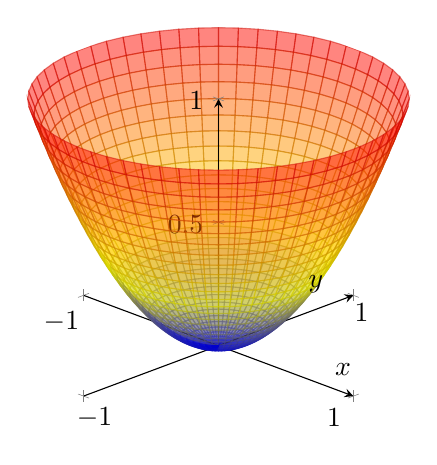
\begin{tikzpicture}

    \begin{axis}[
            view={45}{30},
            axis lines=none,
            xmin=-1, xmax=1,
            ymin=-1, ymax=1,
            zmin=0, zmax=1,
        ]
        \addplot3[
            surf,
            samples=31,                            
            opacity = 0.5,
            domain=0:1,y domain=45:225,
            z buffer=sort,
        ]
        ({x * cos(y)},
        {x * sin(y)},
        x^2);
    \end{axis}
    \begin{axis}[
            view={45}{30},
            xlabel=\(x\), ylabel=\(y\),
            axis lines=center,
            xmin=-1, xmax=1,
            ymin=-1, ymax=1,
            zmin=0, zmax=1,
        ]
        \addplot3[
            surf,
            samples=31,
            opacity = 0.5,
            domain=0:1,y domain=225:405,
            z buffer=auto,
        ]
        ({x * cos(y)},
        {x * sin(y)},
        x^2);
    \end{axis}
\end{tikzpicture}

\end{document}